\documentclass{beamer}
\usepackage[utf8]{inputenc}
\usepackage[brazilian]{babel}
\usepackage{graphicx}
\usepackage{tikz}
\usepackage{hyperref}

\usetheme{Madrid}
\usecolortheme{default}

\title{Projeto IcarUSP: Sistema de Catalogação e Busca de Livros}
\subtitle{Relatório de Progresso - Ciclo 2}
\author{Isabela Miki \& Jonas Rodrigues}
\date{\today}

\begin{document}

\begin{frame}
\titlepage
\end{frame}

\begin{frame}{Sistema Dedalus da USP}
\begin{center}
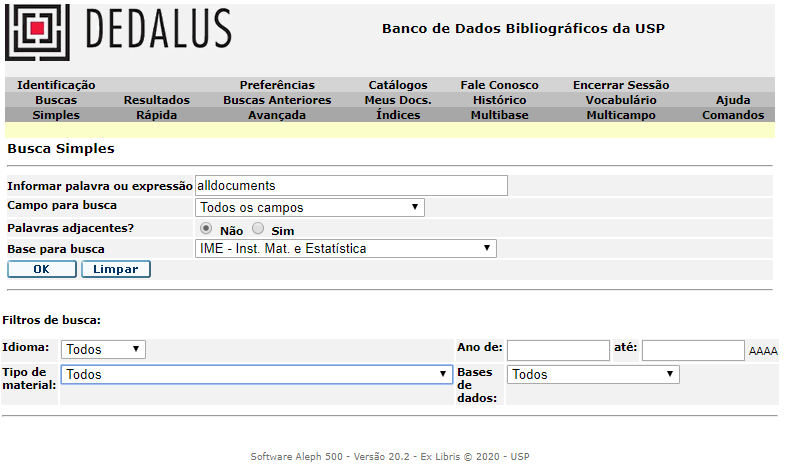
\includegraphics[width=0.8\textwidth]{dedalus.png}
\end{center}
\vspace{0.5cm}
\begin{itemize}
\item Sistema atual de catalogação e busca de livros da USP
\item Interface complexa e antiga
\item Funcionalidades dispersas
\end{itemize}
\end{frame}

\begin{frame}{Propósito do Sistema Icarus}
\begin{itemize}
\item \textbf{Problema identificado:} O Dedalus possui interface complexa e
busca limitada, dificultando a localização eficiente de materiais acadêmicos
\item \textbf{Solução proposta:} Sistema simplificado para catalogação e busca
de livros e papers com interface intuitiva
\item \textbf{Escopo:}
    \begin{itemize}
    \item Cadastro e consulta de autores, livros e papers
    \item Busca por similaridade utilizando tecnologia de busca vetorial
    \item Sistema simplificado focado nas principais funcionalidades
    \end{itemize}
\end{itemize}
\end{frame}

\begin{frame}{Diagrama de Classes}
\begin{center}
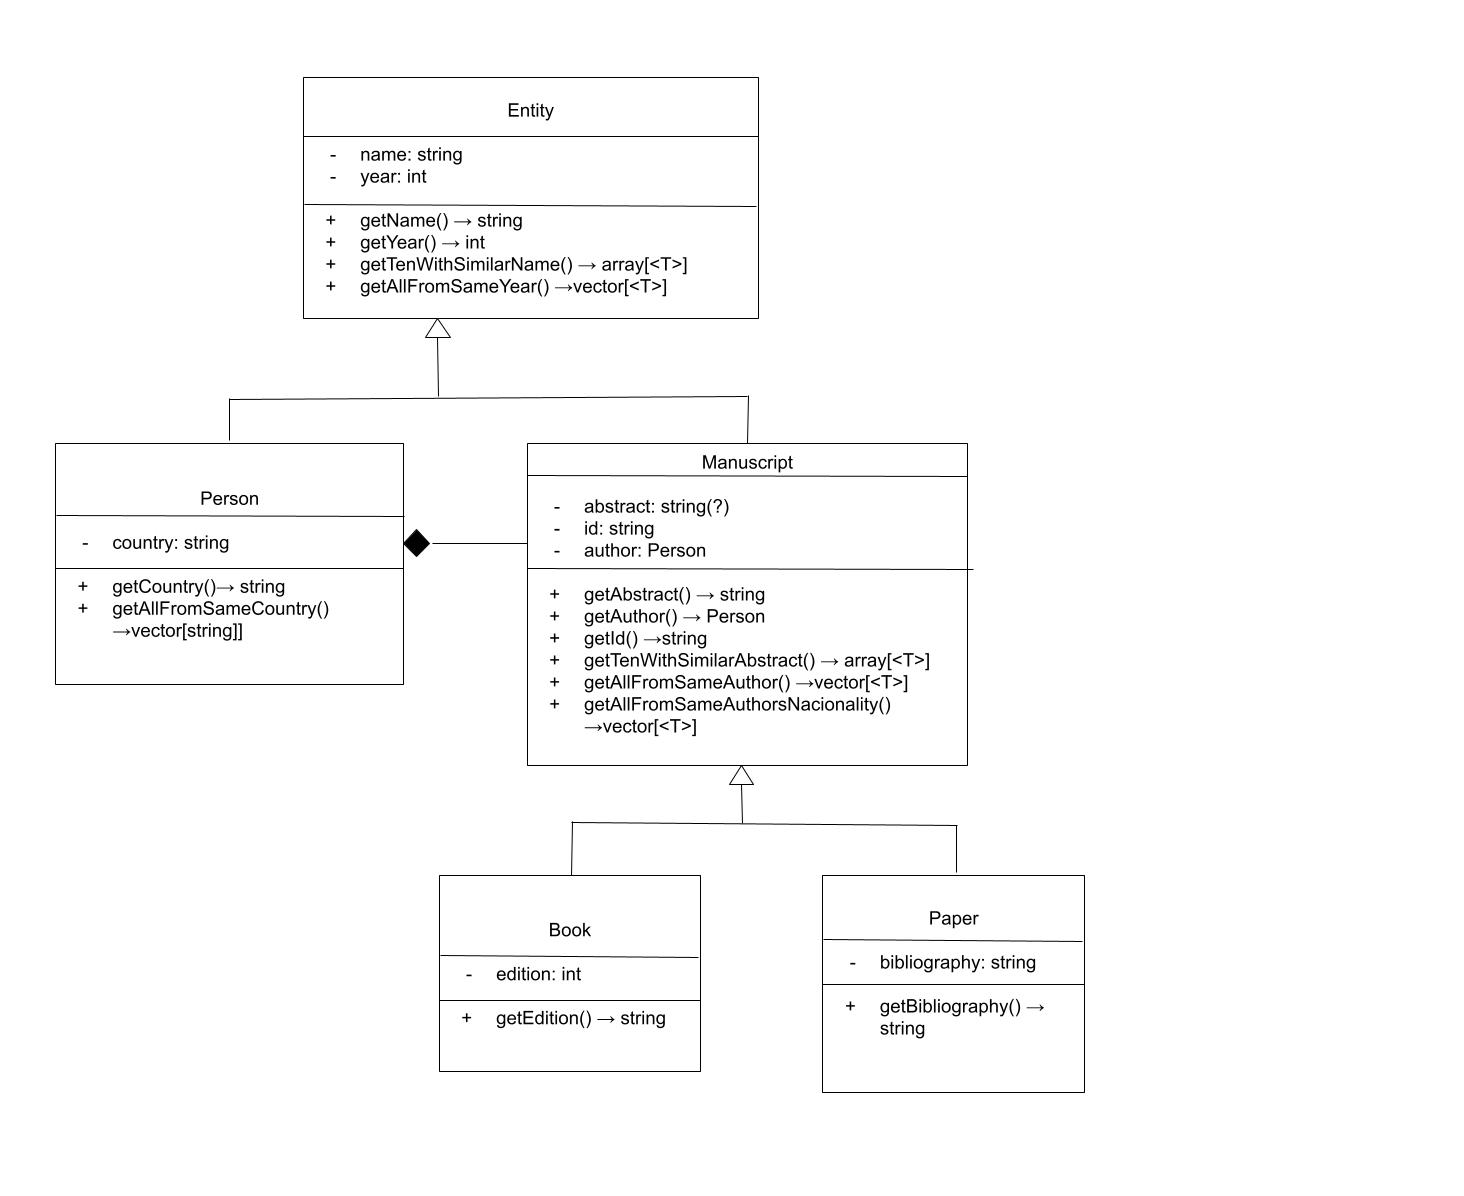
\includegraphics[width=0.9\textwidth]{../UML.jpg}
\end{center}
\end{frame}

\begin{frame}{Tecnologias Utilizadas}
\begin{tabular}{ccc}
    \textbf{Frontend} & \textbf{Backend} & \textbf{Banco de Dados} \\
    \begin{minipage}{0.3\textwidth}
        \begin{itemize}
            \item Svelte com TypeScript
            \item Interfaces responsivas
            \item Formulários para cadastro
            \item Componentes de busca intuitivos
        \end{itemize}
    \end{minipage} &
    \begin{minipage}{0.3\textwidth}
        \begin{itemize}
            \item Rust (orientado a objetos)
            \item Alta performance
            \item Segurança de memória
            \item Processamento dos embeddings (via integração com Torch)
        \end{itemize}
    \end{minipage} &
    \begin{minipage}{0.3\textwidth}
        \begin{itemize}
            \item Limbo (variante SQLite)
            \item Suporte a buscas vetoriais
            \item Leve e de fácil implementação
            \item Não requer infraestrutura complexa
        \end{itemize}
    \end{minipage} \\
\end{tabular}
\end{frame}

\begin{frame}{Busca Vetorial}
\begin{itemize}
\item \textbf{Conceito:} Transformação de texto em vetores numéricos
(embeddings)
\item \textbf{Funcionamento:}
\begin{enumerate}
\item O resumo de um livro é convertido em um vetor numérico
\item Vetores similares representam conteúdos semanticamente próximos
\item A busca encontra os vetores mais próximos ao da consulta
\end{enumerate}
\item \textbf{Vantagem:} Encontra livros com conteúdo similar mesmo quando as
palavras exatas não são as mesmas
\end{itemize}
\vspace{0.5cm}
\begin{center}
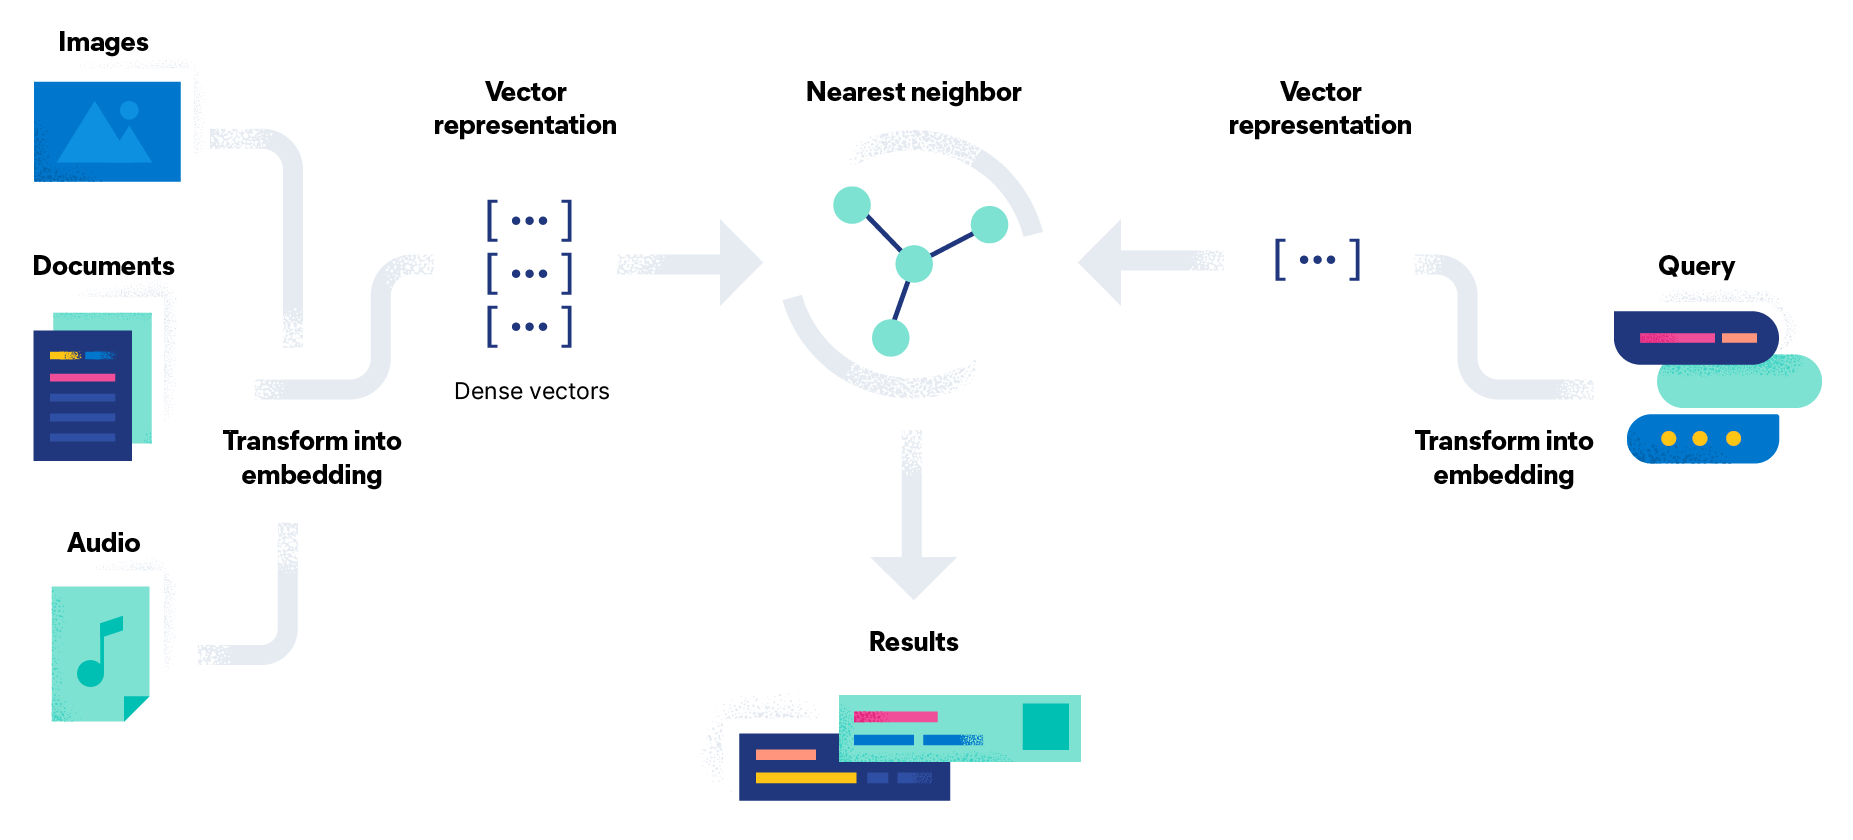
\includegraphics[width=0.7\textwidth]{vector_search.png}
\end{center}
\end{frame}

\begin{frame}{Próximos Passos}
\begin{itemize}
\item Finalizar a integração do backend com o banco de dados Limbo
\item Implementar o algoritmo de busca vetorial
\item Desenvolver a interface de usuário para cadastro e consulta
\item Criar testes automatizados para garantir cobertura de 90\%
\item Integrar frontend e backend através de API REST
\end{itemize}
\end{frame}

\end{document}
